\subsection{Prototyping}

Nachdem mithilfe der Nutzwertanalyse im Kapitel \ref{nutzwertanalyse} ein grundlegendes Gesamtkonzept festgelegt wurde, wird nun an Prototypen der einzelen Teilfunktionen gearbeitet. Das Ziel ist es, die einzelnen Teilfunktionen zu Testen und möglichst viele Fehler frühzeitig zu erkennen. Detaillierte Prototypen helfen die bereits bekannten Risiken besser einzuschätzen und neue Risiken frühzeitig zu erkennen.

\subsubsection{Greifer-Prototyp I}
\label{subsubsection:gripper-prototype-1}


Der Aufbau und die Funktionsweise des Greifers werden in Kapitel \ref{subsubsection:Hindernisse bewegen} erläutert. Um die Auslegung des Greifers \textbf{(REF AUSLEGUNG)} zu validieren und sein Funktionsprinzip zu überprüfen wurde ein Prototyp gebaut (Abb. \ref{fig:gripper-prototype-trimetric-notes}). Der Prototyp besthet abgesehenen von den Schrauben aus 3D-Druck Komponenten. der Aufbau wurde so gewählt, dass Iterationen an Einzelteilen schnell realisiert und verbaut werden können. 

\begin{figure}[H]
\centering
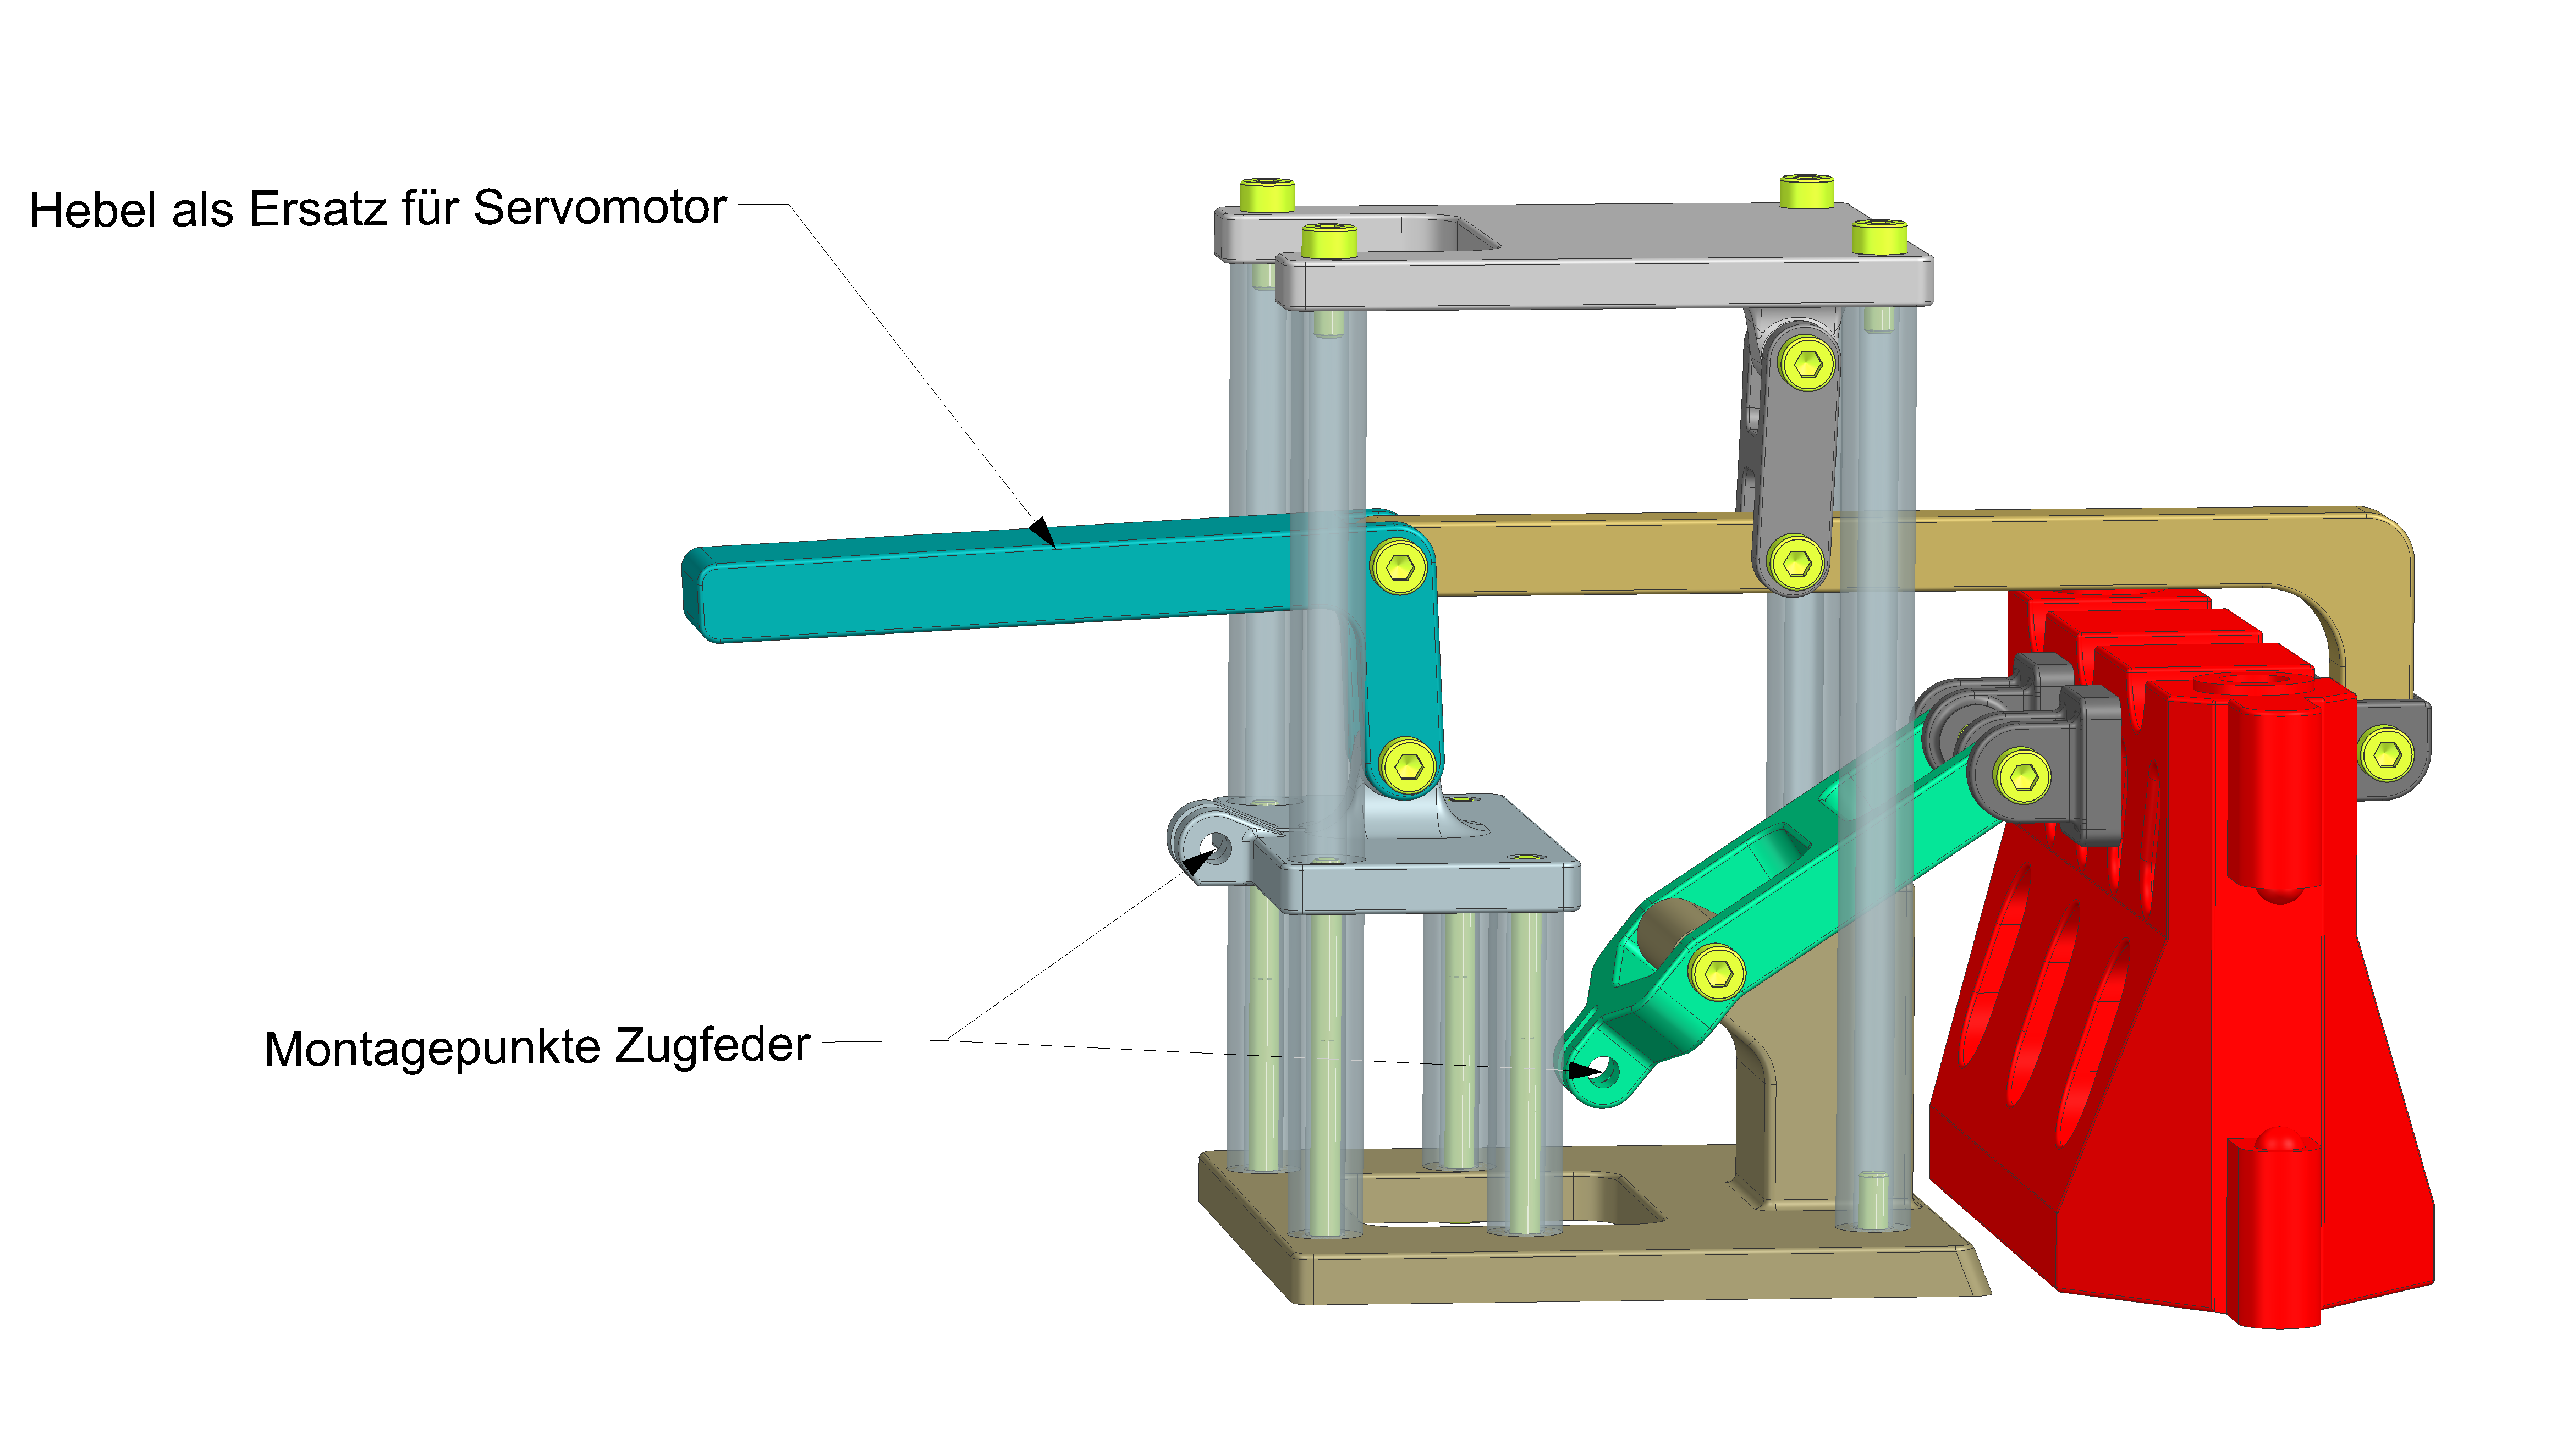
\includegraphics[width=1.0\textwidth]{assets/greifer-prototyp/Greifer_Trimetrisch_Notes.png}
\caption{Prototyp Greifer}
\label{fig:gripper-prototype-trimetric-notes}
\end{figure}

\newpage

Mit dem Prototyp sollen folgenden Punkte getestet werden können:
\begin{itemize}
    \item Das Gestänge funktioniert wie konstruiert (Gelenke sind freigängig, keine Kollisionen)
    \item Das Gestänge verklemmt im Betrieb nicht 
    \item Hindernis kann zuverlässig angehoben werden. (Stärke der Zugfeder, Reibung an Backen ausreichend)
    \item Hindernis kann auch bei bis zu 15° Schrägstellung angehoben werden
    \item Hindernis wird zuverlässig an dieselbe Stelle zurückgesetzt
    \item Hindernis rutscht nicht aus dem Greifer bei Vibrationen des Fahrzeugs
    \item  Nötiges Drehmoment zum Anheben entspricht dem ausgelegten Drehmoment
\end{itemize}

Der Prototyp des Greifers wird Manuell über einen Heble bedient, welcher anstelle des Servomotors in der Konstruktion verbaut ist. Diese Entscheideung wurde getroffen, da das ausgelegte Motordrehmoment durch mögliche Reibung in den Gelenken nicht ausreichen könnte. Mit dem Hebel kann das Moment einfach durch aufbringen einer bekannten Last validiert werden.
\\
Die Lagerpunkte des Gestänges wurden für den Prototyp an ein Gestell aufgebracht (Abb. \ref{fig:gripper-frame-mounting-points}). So kann der Greifer unabhängig vom Fahrzeug getestet werden. Die Abstände zwischen den Lagerpunkten sowie zum Boden sollen für den finalen Greifer dieselben sein. Auch die Dimensionen des Gestänges sollen beibehalten werden (Abb. \ref{fig:gripper-linkage-dimensions}). Somit bleiben die von der Geometrie abhängigen Kräfte dieselben und Ergebnisse aus Prototypentests können auf spätere Iterationen übertragen werden.

\begin{figure}[H]
\begin{subfigure}{0.9\textwidth}
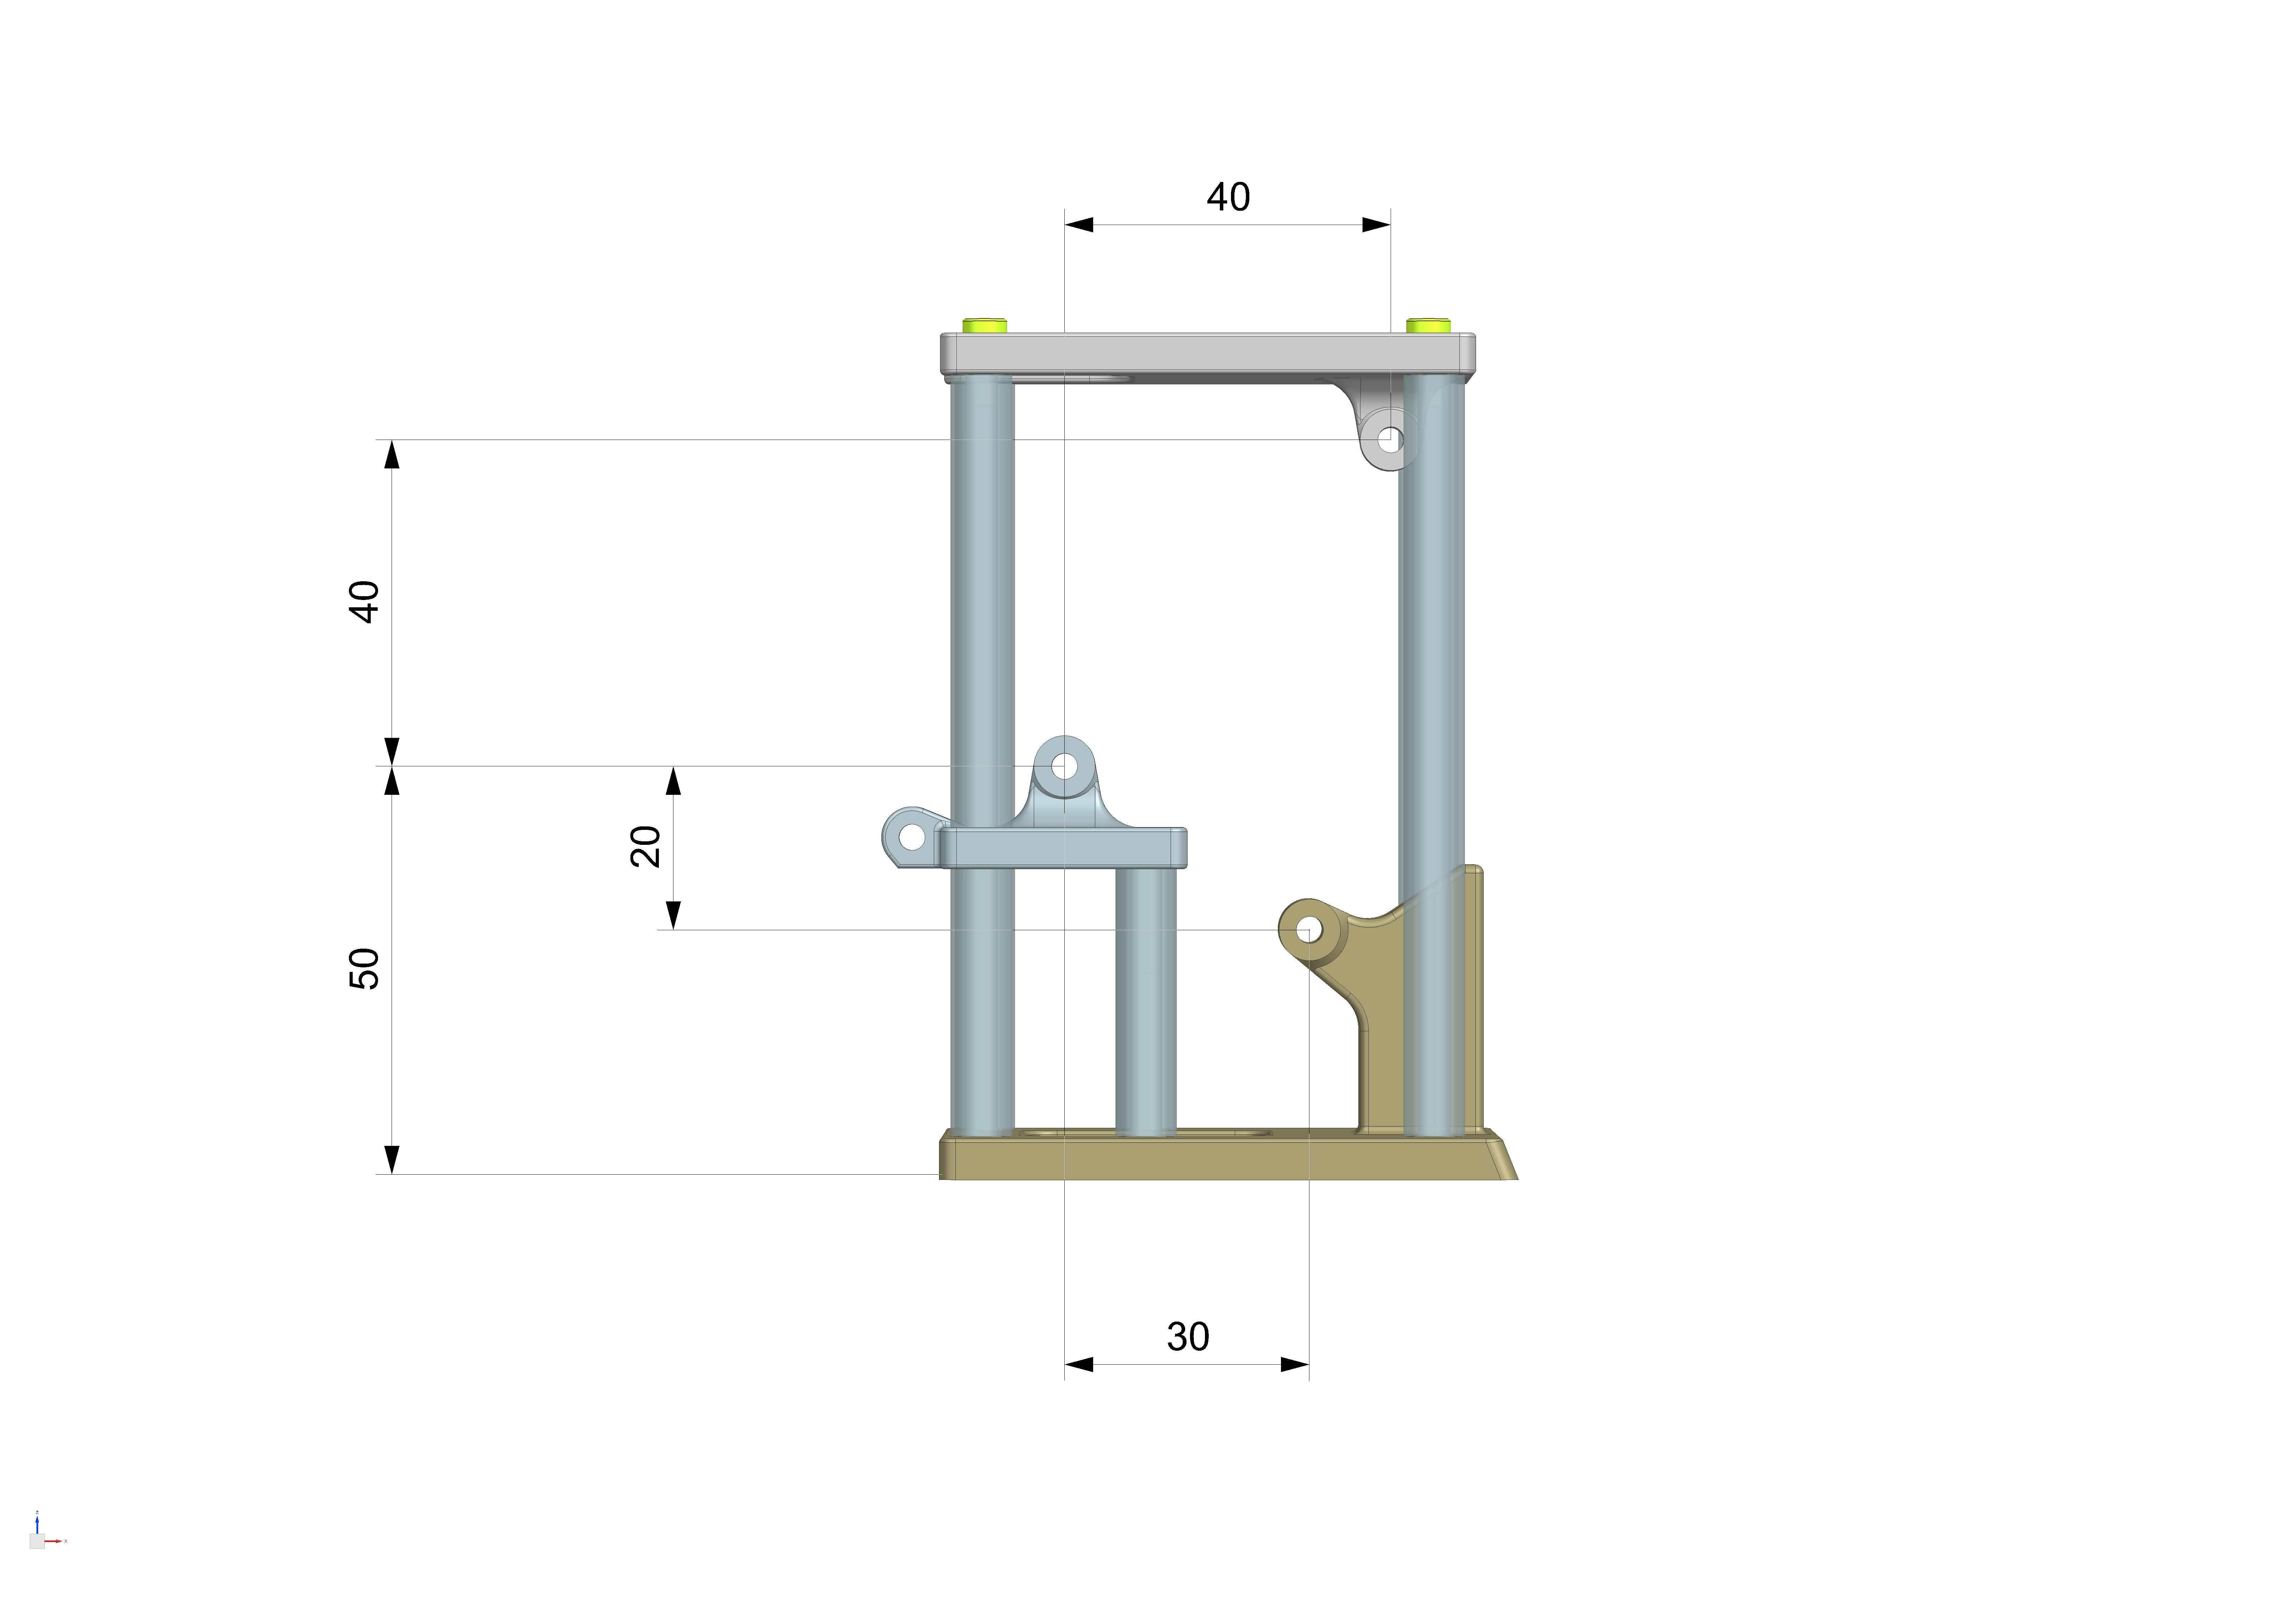
\includegraphics[width=\textwidth]{assets/greifer-prototyp/Greifer_Dimensionen_Lagerpunkte.png}
\caption{Gestell mit Lagerpunkten}
\label{fig:gripper-frame-mounting-points}
\end{subfigure}
\begin{subfigure}{0.9\textwidth}
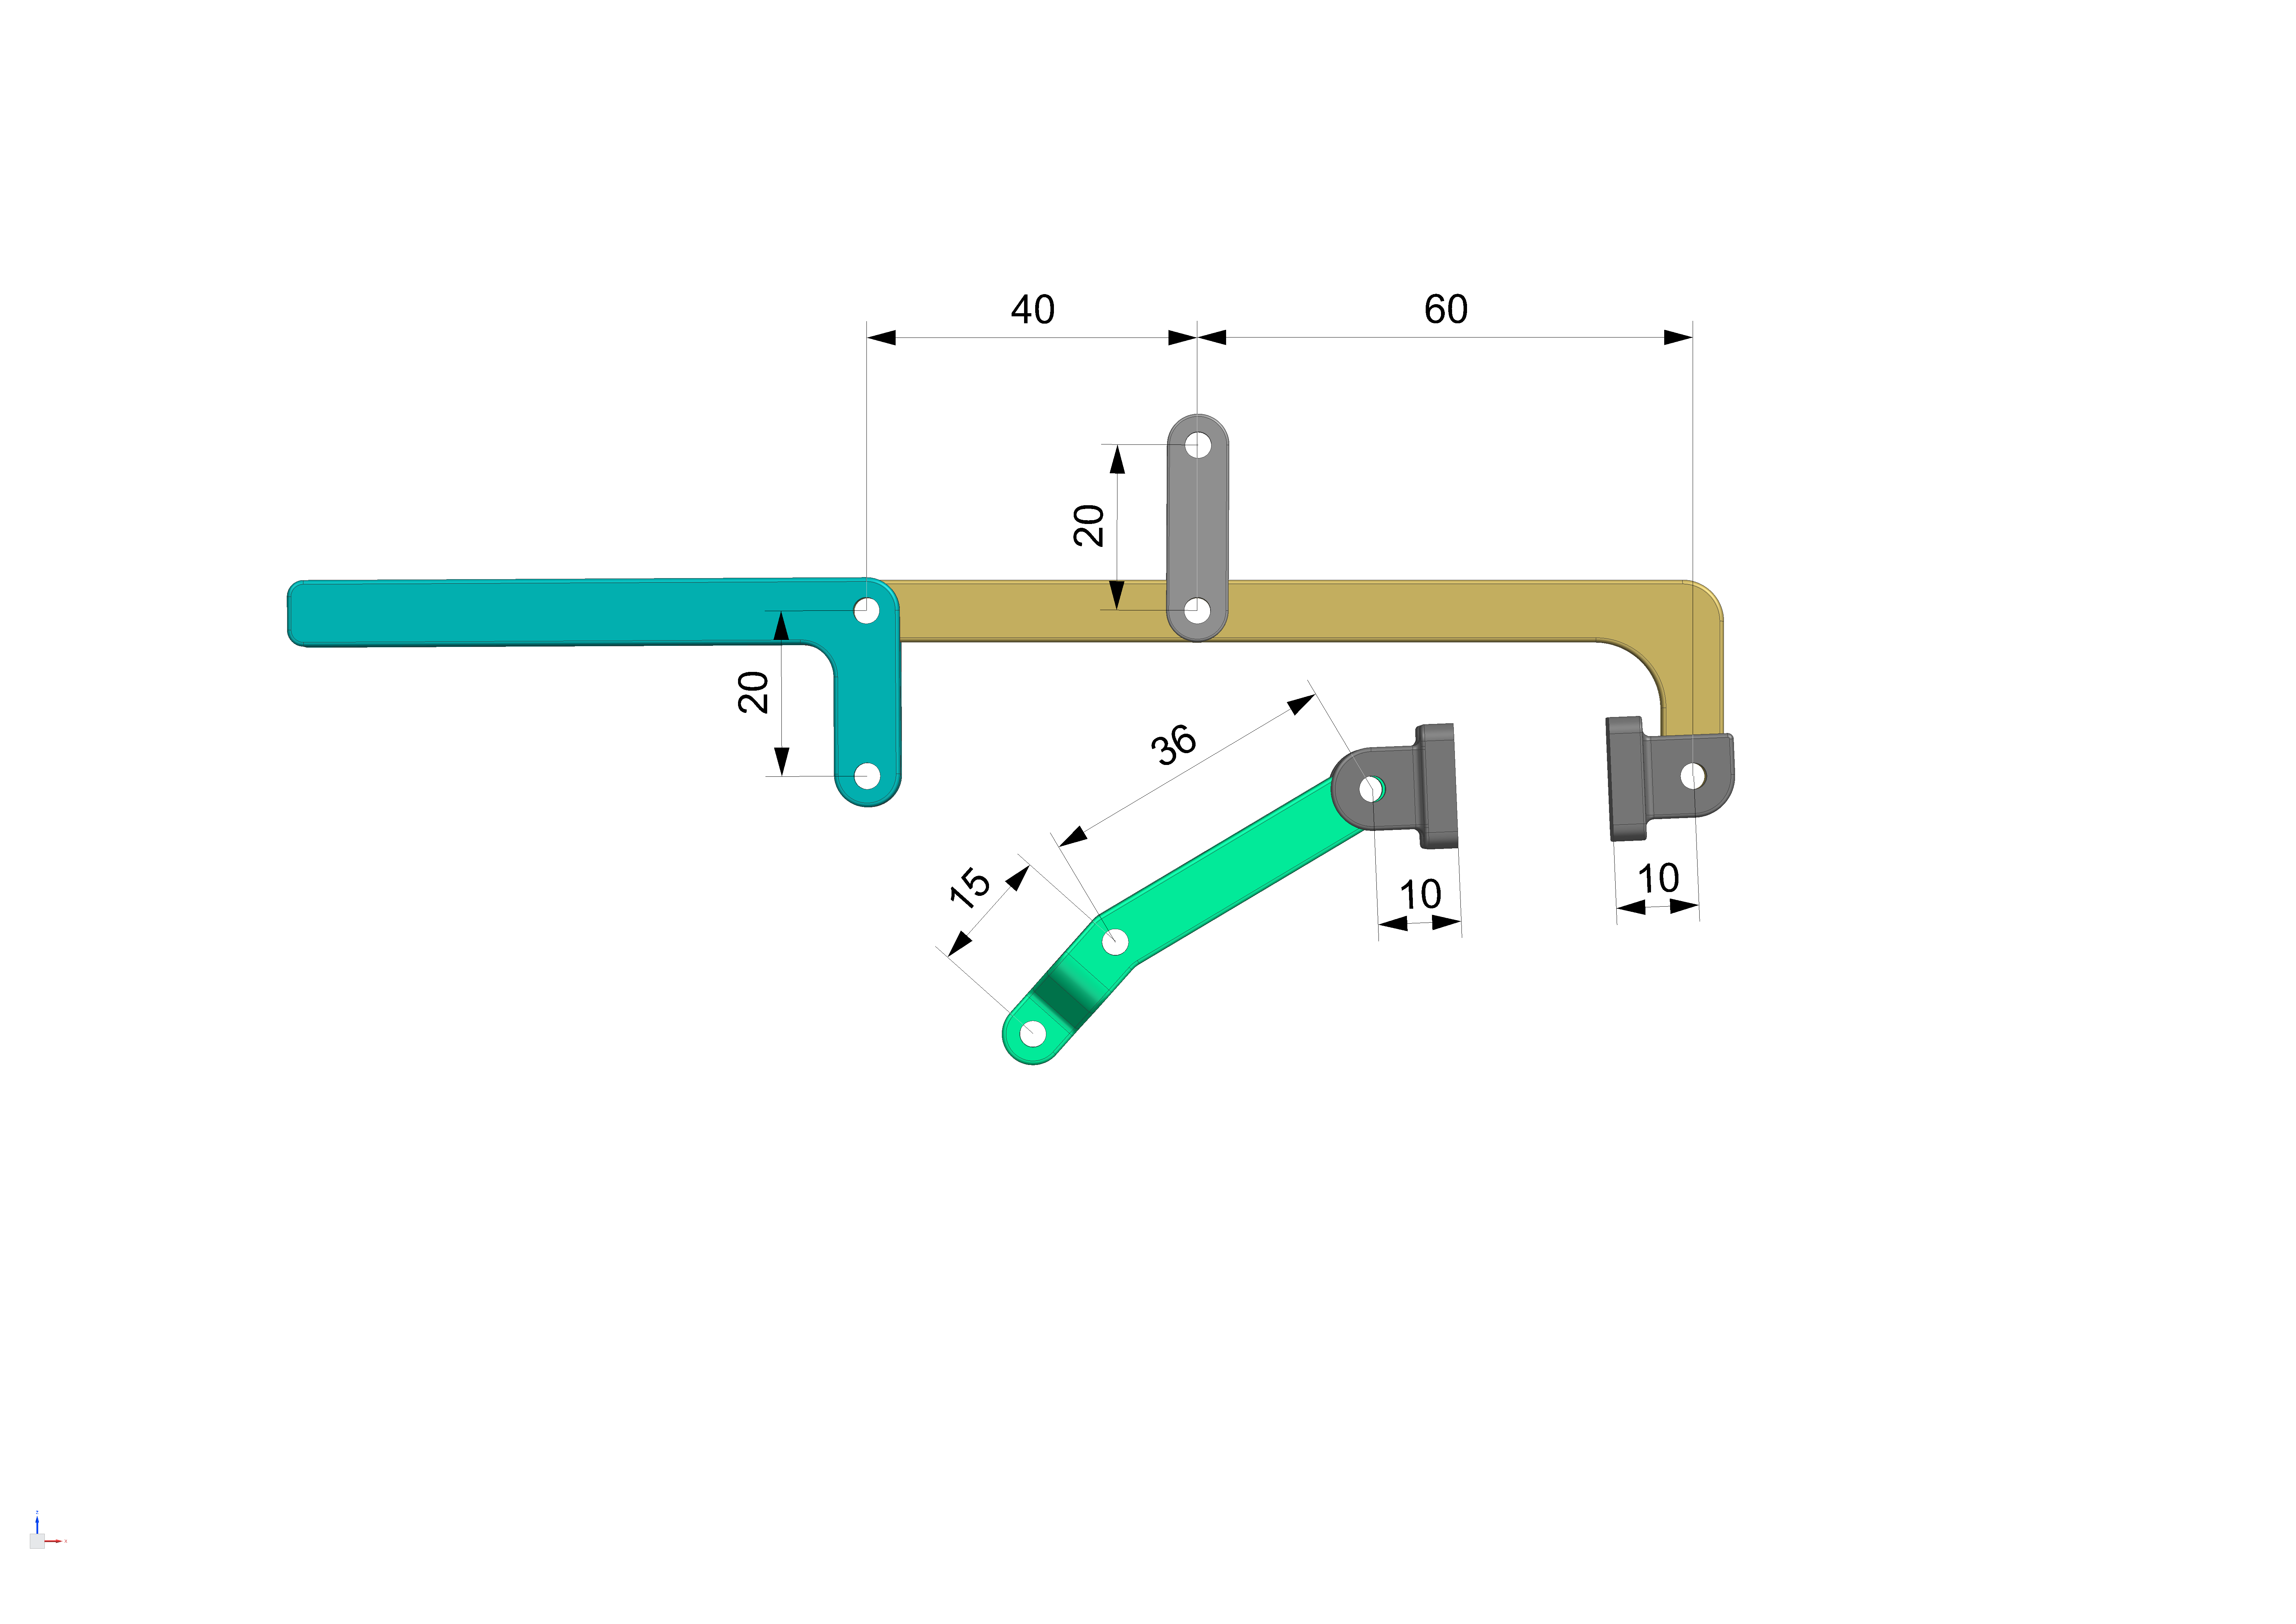
\includegraphics[width=\textwidth]{assets/greifer-prototyp/Greifer_Dimensionen_Arme.png}
\caption{Dimensionen des Gestänges}
\label{fig:gripper-linkage-dimensions}
\end{subfigure}
\caption{Dimensionen Prototyp}
\label{gripper-prototype-dimensions}
\end{figure}

\subsubsection{Fahrwerk}

Auf Basis des Gesamtkonzepts wurde anschliessend ein Prototyp für das Fahrwerk konstruiert. Die Baugruppe Prototyp Fahrwerk beinhaltet alle für die selbständige Fortbewegung notwendigen Elemente wie Motoren, Akkus, Liniensensoren und Steuerungseinheiten.  Bei diesem Prototyp stand der einfache und zweckmässige Aufbau im Vordergrund. Bei der Grundplatte wurde darauf geachtet das verschiedene  Versionen von Systemen einfach aufgebaut und ausgetauscht werden können. Ein flexibeler Prototyp ist Ressourcenschonend. Mehr Informationen im Kapitel \ref{section:Nachhaltigkeit} Nachhaltigkeit. 
